\documentclass{article}

\usepackage[letterpaper, portrait, margin=1.5in]{geometry}

\usepackage{fancyhdr}
\usepackage{ragged2e}
\usepackage{graphicx}
\usepackage{caption}
\usepackage{amsmath}
\usepackage{rotating}

\usepackage{listings}
\usepackage{color}
\usepackage{caption}
\usepackage{subcaption}

\definecolor{dkgreen}{rgb}{0,0.6,0}
\definecolor{gray}{rgb}{0.5,0.5,0.5}
\definecolor{mauve}{rgb}{0.58,0,0.82}

\lstset{frame=tb,
  language=Java,
  aboveskip=3mm,
  belowskip=3mm,
  showstringspaces=false,
  columns=flexible,
  basicstyle={\small\ttfamily},
  numbers=none,
  numberstyle=\tiny\color{gray},
  keywordstyle=\color{blue},
  commentstyle=\color{dkgreen},
  stringstyle=\color{mauve},
  breaklines=true,
  breakatwhitespace=true,
  tabsize=4
}

\setcounter{secnumdepth}{1}

\usepackage{chngcntr}
\counterwithin{figure}{section}

\renewcommand*{\thepage}{C\arabic{page}}

\pagestyle{fancy}
\lhead{ACME Robotics}
\chead{\#8367}
\rhead{\ifcontents Contents \else Week \thesection \fi}

\newif\ifcontents
\contentstrue

\makeatletter
\renewcommand{\@seccntformat}[1]{}
\makeatother
\begin{document}
\subsection{Re-wiring Robot}
%! entry 
The team feels its a good practice to have wiring as organized and clear as possible to help with repair, and the over all aesthetics of the robot. This became very evident after an incident that happen last year at Super Regionals in Spokane. There, we ended up having an entire rev hub die due to static, and less than 40 minutes to replace it. But due to our poor wiring job and lack of labeling created a very panicked last minute switch rather than and easy one. \\

Which is why after all the subsystems were on and tested on the current wiring, Oren stripped all the wiring to start over. Being sure to label both ends of all the wires, along with running similar wires as a group to help separate between servo wires, encoder wires, and motor wires. Oren also made sure to place wire connections/extensions in accessible locations, in the off chance they failed or needed to be tested. Oren also used sheathing to cover the wires so they wouldn't get caught by any moving component, along with creating a cleaner aesthetic for the over all robot. 

\subsection{Changing the Marker Deployment Mechanism}
%@ entry
Since the teams goal for Worlds was to run cycles in auto, they needed to shorten the time required for claiming the depot. The easiest way to do this was to drop the marker from the end of the rake, allowing the robot to only get within four feet of the depot. This would significantly reduce the time allotted for claiming in auto, allowing for more cycles. To drop from the rake the mechanism needed to be reliable without possibly getting flung out of the depot. The problematic factor was that the space at the end of the rake was minimal because it was already almost at the 18 mark. To do this Kelly, Aidan, and Jon brainstormed possible solutions. The original result in week 27 proved to be ineffective. After more brainstorming the result was a three piece mechanism as shown in figure \ref{fig:MDM}. The mechanism involved a slide part mounted on the X-Rail slides, a key on the marker that fit into the slide, and a metal bar that was attached to the rake and ran through the key. When the rake was rotated down the key would no longer hold the marker up and the marker would fall from the slide piece. The team was satisfied with the mechanism because it held the marker in place with support from all directions and always dropped the marker in the desired spot without error.


\begin{figure}[h!]
\centering
\begin{subfigure}{.45\textwidth}
  \centering
  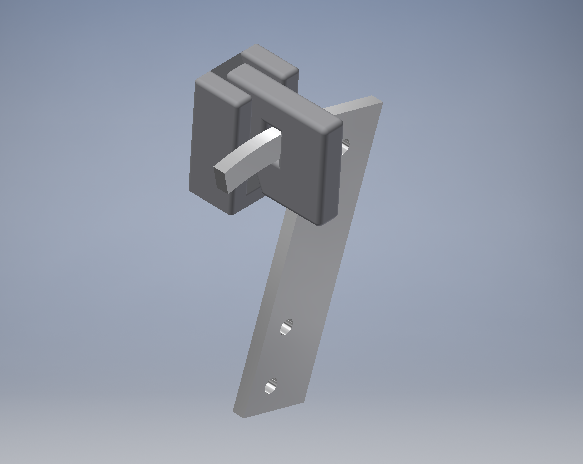
\includegraphics[width=1\textwidth]{29_03-18/images/marker.png}
  \caption{Marker Deployment Mechanism CAD}
  \label{fig:MDM}
 \end{subfigure}
\begin{subfigure}{.45\textwidth}
  \centering
  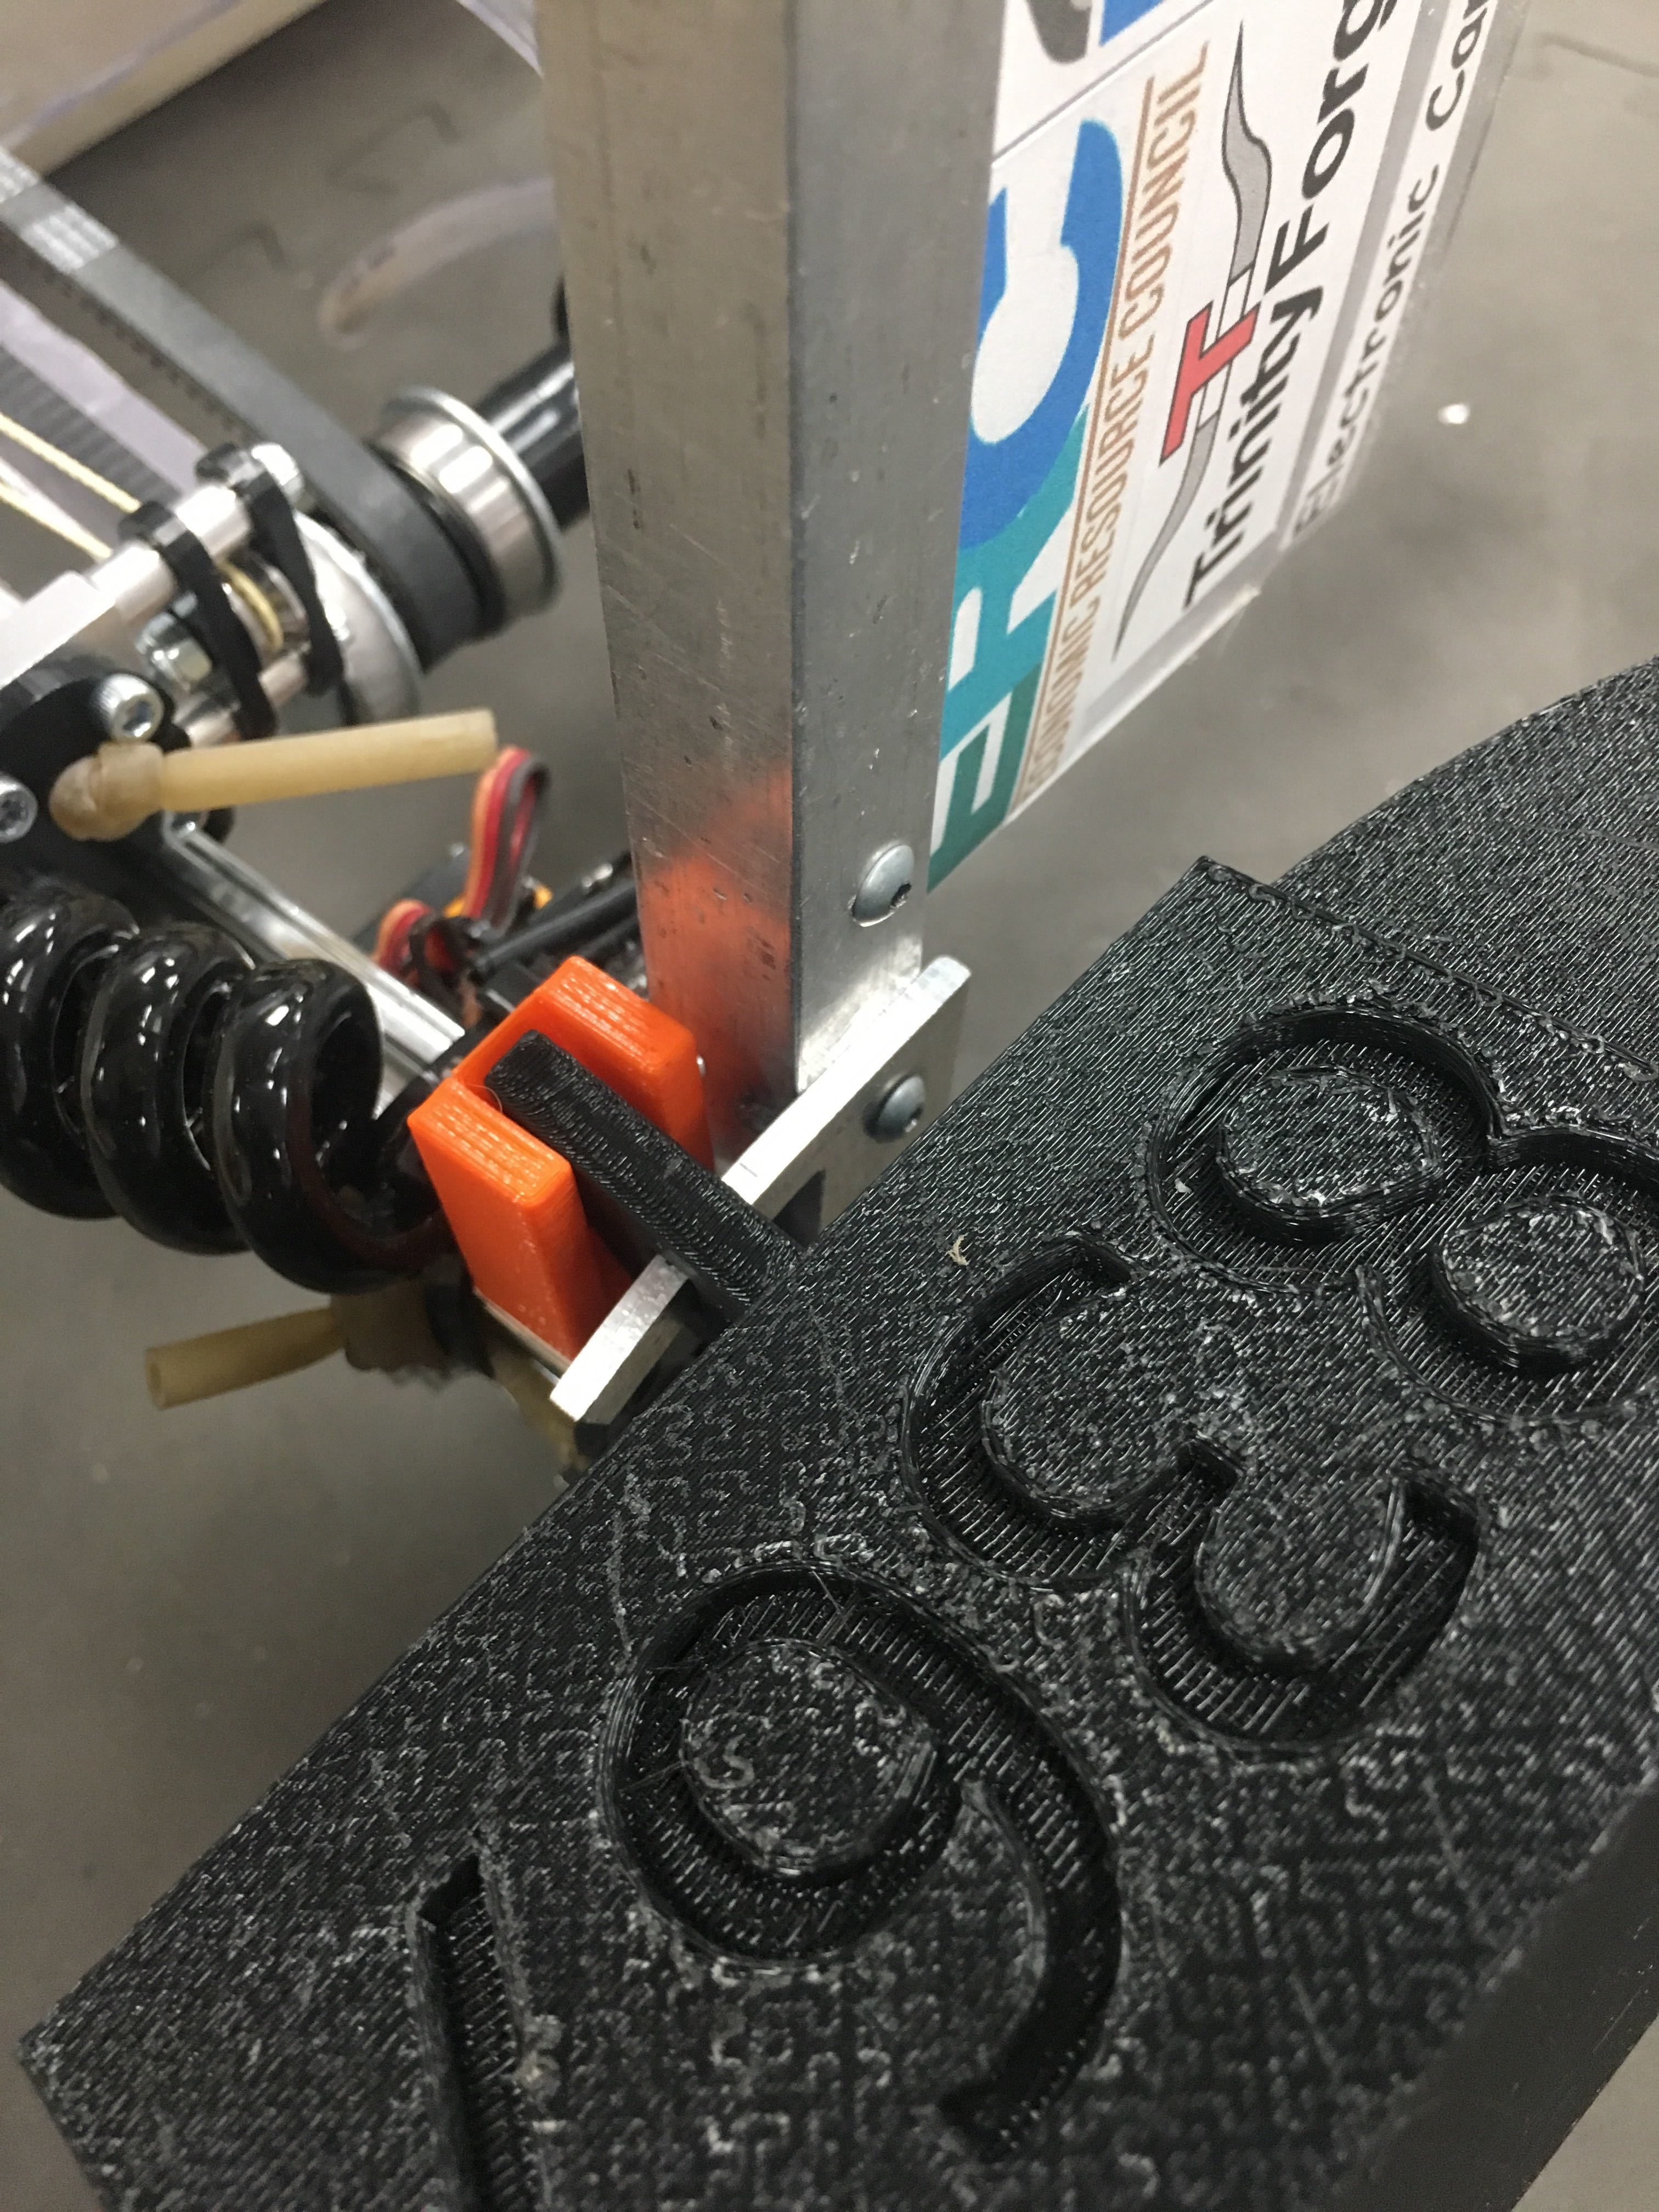
\includegraphics[width=.75\textwidth]{29_03-18/images/thing.jpg}
  \caption{Marker Deployment Mechanism}
  \label{fig:hub}
  \end{subfigure}
  \caption{Marker Deployment Mechanism}
  \end{figure}

\end{document}